% This is a Basic Assignment Paper but with like Code and stuff allowed in it, there is also url, hyperlinks from contents included. 

\documentclass[11pt]{article}

% Preamble

\usepackage[margin=1in]{geometry}
\usepackage{amsfonts, amsmath, amssymb}
\usepackage{fancyhdr, float, graphicx}
\usepackage[utf8]{inputenc} % Required for inputting international characters
\usepackage[T1]{fontenc} % Output font encoding for international characters
\usepackage{fouriernc} % Use the New Century Schoolbook font
\usepackage[nottoc, notlot, notlof]{tocbibind}
\usepackage{listings}
\usepackage{xcolor}
\usepackage{blindtext}
\usepackage{hyperref}
\hypersetup{
    colorlinks=true,
    linkcolor=black,
    filecolor=magenta,      
    urlcolor=cyan,
    pdfpagemode=FullScreen,
    }

\definecolor{codegreen}{rgb}{0,0.6,0}
\definecolor{codegray}{rgb}{0.5,0.5,0.5}
\definecolor{codepurple}{rgb}{0.58,0,0.82}
\definecolor{backcolour}{rgb}{0.95,0.95,0.92}

\lstdefinestyle{mystyle}{
    backgroundcolor=\color{backcolour},   
    commentstyle=\color{codegreen},
    keywordstyle=\color{magenta},
    numberstyle=\tiny\color{codegray},
    stringstyle=\color{codepurple},
    basicstyle=\ttfamily\footnotesize,
    breakatwhitespace=false,         
    breaklines=true,                 
    captionpos=b,                    
    keepspaces=true,                 
    numbers=left,                    
    numbersep=5pt,                  
    showspaces=false,                
    showstringspaces=false,
    showtabs=false,                  
    tabsize=2
}

\lstset{style=mystyle}

% Header and Footer
\pagestyle{fancy}
\fancyhead{}
\fancyfoot{}
\fancyhead[L]{\textit{\Large{Philosophy of Science and Religion - Second Year B. Tech, Semester 2}}}
%\fancyhead[R]{\textit{something}}
\fancyfoot[C]{\thepage}
\renewcommand{\footrulewidth}{1pt}



% Other Doc Editing
% \parindent 0ex
%\renewcommand{\baselinestretch}{1.5}

\begin{document}

\begin{titlepage}
	\centering

	%---------------------------NAMES-------------------------------

	\huge\textsc{
		MIT World Peace University
	}\\

	\vspace{0.75\baselineskip} % space after Uni Name

	\LARGE{
		Philosophy of Science and Religion\\
		Second Year B. Tech, Semester 1
	}

	\vfill % space after Sub Name

	%--------------------------TITLE-------------------------------

	\rule{\textwidth}{1.6pt}\vspace*{-\baselineskip}\vspace*{2pt}
	\rule{\textwidth}{0.6pt}
	\vspace{0.75\baselineskip} % Whitespace above the title



	\huge{\textsc{
			"Science without religion is lame, religion without science is blind"\\
			And "A short note and Christianity"
		}} \\



	\vspace{0.5\baselineskip} % Whitespace below the title
	\rule{\textwidth}{0.6pt}\vspace*{-\baselineskip}\vspace*{2.8pt}
	\rule{\textwidth}{1.6pt}

	\vspace{1\baselineskip} % Whitespace after the title block

	%--------------------------SUBTITLE --------------------------	

	\LARGE\textsc{
		Assignment 1
	} % Subtitle or further description
	\vfill

	%--------------------------AUTHOR-------------------------------

	Prepared By
	\vspace{0.5\baselineskip} % Whitespace before the editors

	\Large{
		Krishnaraj Thadesar \\
		Cyber Security and Forensics\\
		Batch A1, PA 20
	}


	\vspace{0.5\baselineskip} % Whitespace below the editor list
	\today
	
\end{titlepage}


\tableofcontents
\thispagestyle{empty}
\clearpage

\setcounter{page}{1}

\begin{quotation}
	"Science without religion is lame, religion without science is blind" - Albert Einstein\\
	and "A short Note on Christianity"
\end{quotation}

\begin{figure}[H]
	\centering
	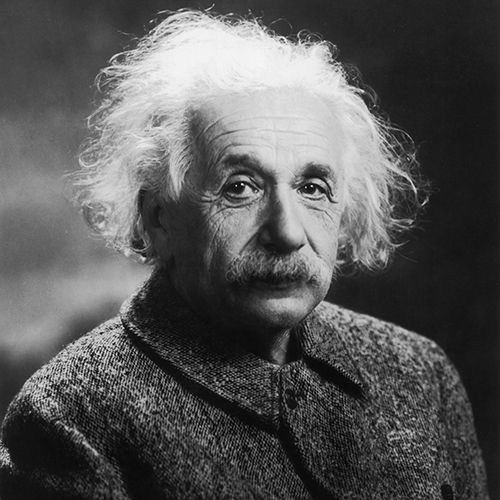
\includegraphics[width=.45\textwidth]{gettyimages-3091504.jpg}
	\caption{Albert Einstein}
\end{figure}

\section{Question A}

\subsection{Science and Religion: Complementary Forces}

"Science without religion is lame, religion without science is blind" is a statement that highlights the interplay between science and religion. While the two are often seen as conflicting forces, they can also complement each other to provide a holistic understanding of the world.\\

Science is concerned with empirical evidence, reason, and the physical world. It provides us with knowledge and understanding of the universe and has made remarkable progress in the last few centuries. However, science alone cannot answer all of life's big questions. For example, science cannot provide answers to questions like the meaning of life or the nature of morality. Religion, on the other hand, is concerned with the spiritual and emotional needs of human beings. It offers a framework for understanding the world beyond the physical realm and can provide us with a sense of meaning and purpose.\\

Religion and science have different strengths and limitations, but they can complement each other. Science provides us with knowledge about the physical world, while religion offers a sense of purpose and direction. Together, they offer a more complete understanding of the world around us.

\begin{figure}[H]
	\centering
	\includegraphics[width=.45\textwidth]{DALL·E 2023-04-12 21.26.48 - Albert Einstein as a Conflicted individual between science and religion.png}
	\caption{Albert Einstein depicted as a person confused between science and Religion}
\end{figure}

\subsection{The Limitations of Science and Religion}

While science and religion can complement each other, they also have their limitations. Science is concerned with the physical world and empirical evidence, but it cannot answer questions about the spiritual realm. Religion, on the other hand, can offer comfort and guidance, but it cannot provide us with empirical evidence or scientific knowledge.\\

Science can also be limited by its methodology. Science relies on the scientific method, which is based on observation, experimentation, and verification. This means that not all questions can be answered by science, as some phenomena may be difficult to observe or test. Additionally, scientific knowledge is constantly evolving, which means that our understanding of the world is always subject to change.\\

Religion can also be limited by its reliance on faith and tradition. While faith can be a powerful force, it can also lead to dogmatism and close-mindedness. Additionally, religions often have conflicting beliefs and practices, which can lead to conflicts and misunderstandings.

\subsection{Examples of the Complementarity of Science and Religion}

Despite their limitations, science and religion can complement each other, as illustrated by various examples from real life. For example, the work of Mother Teresa and Martin Luther King Jr. was guided by their religious beliefs. Mother Teresa, a Catholic nun, dedicated her life to serving the poor and believed that serving others was a way of serving God. Martin Luther King Jr., a Baptist minister, was a leader of the civil rights movement and believed that all people were equal in the eyes of God.\\

Science and religion can also complement each other in the field of medicine. While medicine has made remarkable progress in curing physical ailments, it often neglects the emotional and spiritual needs of patients. Patients who are terminally ill or suffering from chronic pain often turn to religion or spirituality for comfort and solace, which cannot be provided by medicine alone.\\

In conclusion, the statement "Science without religion is lame, religion without science is blind" highlights the interplay between science and religion. While the two are often seen as conflicting forces, they can also complement each other to provide a more complete understanding of the world. Science provides us with knowledge about the physical world, while religion offers a sense of purpose and direction. It is important to acknowledge the limitations of both science and religion and to recognize that they can complement each other in creating a more complete understanding of the world around us.\\


\begin{figure}[H]
	\centering
	\includegraphics[width=.45\textwidth]{DALL·E 2023-04-12 21.30.39 - a lonely robot with AI holding testtube in one hand and a candle in another hand, the robot is praying and also conducting a reaction in his test tube.png}
	\caption{A lonely AI robot holding a test-tube in one hand and a candle in another hand}
\end{figure}

\section{Question B}
\textbf{A Short Note on Christianity}

\begin{figure}[H]
	\centering
	
\includegraphics[width=.45\textwidth]{christianity-gettyimages-121153575.jpg}
	\caption{Christianity}
\end{figure}

\subsection{Origins and Beliefs of Christianity}

Christianity is a monotheistic religion that traces its origins back to the teachings of Jesus Christ. Jesus was born in Bethlehem, which is now part of modern-day Israel, around 4 BC. He began his ministry around the age of 30 and traveled throughout the Middle East, preaching about the love of God and the importance of forgiveness.\\

Christians believe that Jesus is the Son of God and that he came to earth to save humanity from sin. They believe that Jesus was crucified and died for their sins, but that he was resurrected from the dead three days later. Christians believe that through faith in Jesus, they can be forgiven of their sins and have eternal life.

\subsection{Impact of Christianity on the World}

Christianity has had a profound impact on the world throughout history. It has influenced art, music, literature, and philosophy. Some of the greatest works of art and music in human history have been inspired by Christian themes and ideas.\\

Christianity has also played a significant role in social and political movements. In the United States, the civil rights movement of the 1960s was led in part by Christian pastors and leaders who were inspired by their faith to fight for racial justice and equality. Similarly, Christian organizations have played a key role in efforts to combat poverty and hunger around the world.

\subsection{Modern-day Christianity}

Today, Christianity continues to be an important force in the world. While there are many different denominations of Christianity, they all share a common belief in Jesus Christ and his teachings.\\

In many parts of the world, Christianity is growing rapidly. In sub-Saharan Africa, for example, the number of Christians has more than tripled since 1970. Christianity is also growing in some parts of Asia, particularly in countries like South Korea and China.\\

At the same time, Christianity is facing challenges in other parts of the world. In some Western countries, the number of people who identify as Christian is declining, as more people turn away from organized religion. Christianity is also facing persecution in some parts of the world, particularly in countries where it is a minority religion.\\

Despite these challenges, Christianity continues to inspire and motivate people around the world. Christians are working to live out their faith by helping those in need, striving to love others, and working towards social justice and peace.


\end{document}